\documentclass{article}

% Language setting
% Replace `english' with e.g. `spanish' to change the document language
\usepackage{biblatex} %Imports biblatex package
\addbibresource{refs.bib}
\usepackage[english]{babel}
\usepackage{array}
\usepackage{amsmath}
\usepackage{pythonhighlight}
\usepackage{multirow}
\newcolumntype{P}[1]{>{\centering\arraybackslash}p{#1}}
\newcolumntype{M}[1]{>{\centering\arraybackslash}m{#1}}

% Set page size and margins
% Replace `letterpaper' with `a4paper' for UK/EU standard size
\usepackage[letterpaper,top=2cm,bottom=2cm,left=3cm,right=3cm,marginparwidth=1.75cm]{geometry}

\usepackage{amsmath}
\usepackage{graphicx}
\usepackage[colorlinks=true, allcolors=blue]{hyperref}
\usepackage{setspace}
\usepackage{booktabs}
\usepackage[T1]{fontenc}
\usepackage{longtable}
\doublespacing

\begin{document}
\begin{titlepage}

\centering
\scshape
\vspace{\baselineskip}

%
\rule{\textwidth}{1.6pt}\vspace*{-\baselineskip}\vspace*{2pt}
\rule{\textwidth}{0.4pt}

{\Huge \textbf{\textsc{ Tensile Stress-Strain \\
\vspace{15pt}}}}

\rule{\textwidth}{0.4pt}\vspace*{-\baselineskip}\vspace{3.2pt}
\rule{\textwidth}{1.6pt}\vspace{6pt}
\centerline{\textit{University of Illinois at Urbana-Champaign}} 
\centerline{\textit{Department of Nuclear, Plasma, and Radiological Engineering}}
\vspace{1.5\baselineskip}


\large \centerline{\textbf{Author:} Nathan Glaser}
\large \centerline{\textbf{Net-ID:} nglaser3}
\quad

\vfill
\large \centerline{September 25, 2024}
%
\pagenumbering{gobble}
\end{titlepage}

\tableofcontents
\newpage
\pagenumbering{arabic}

\section{Abstract}

\newpage
\section{Introduction}

\newpage
\section{Experimental Methods}

\newpage
\section{Results}

\subsection{Question 1}
\begin{figure}[!h!]
    \centering
    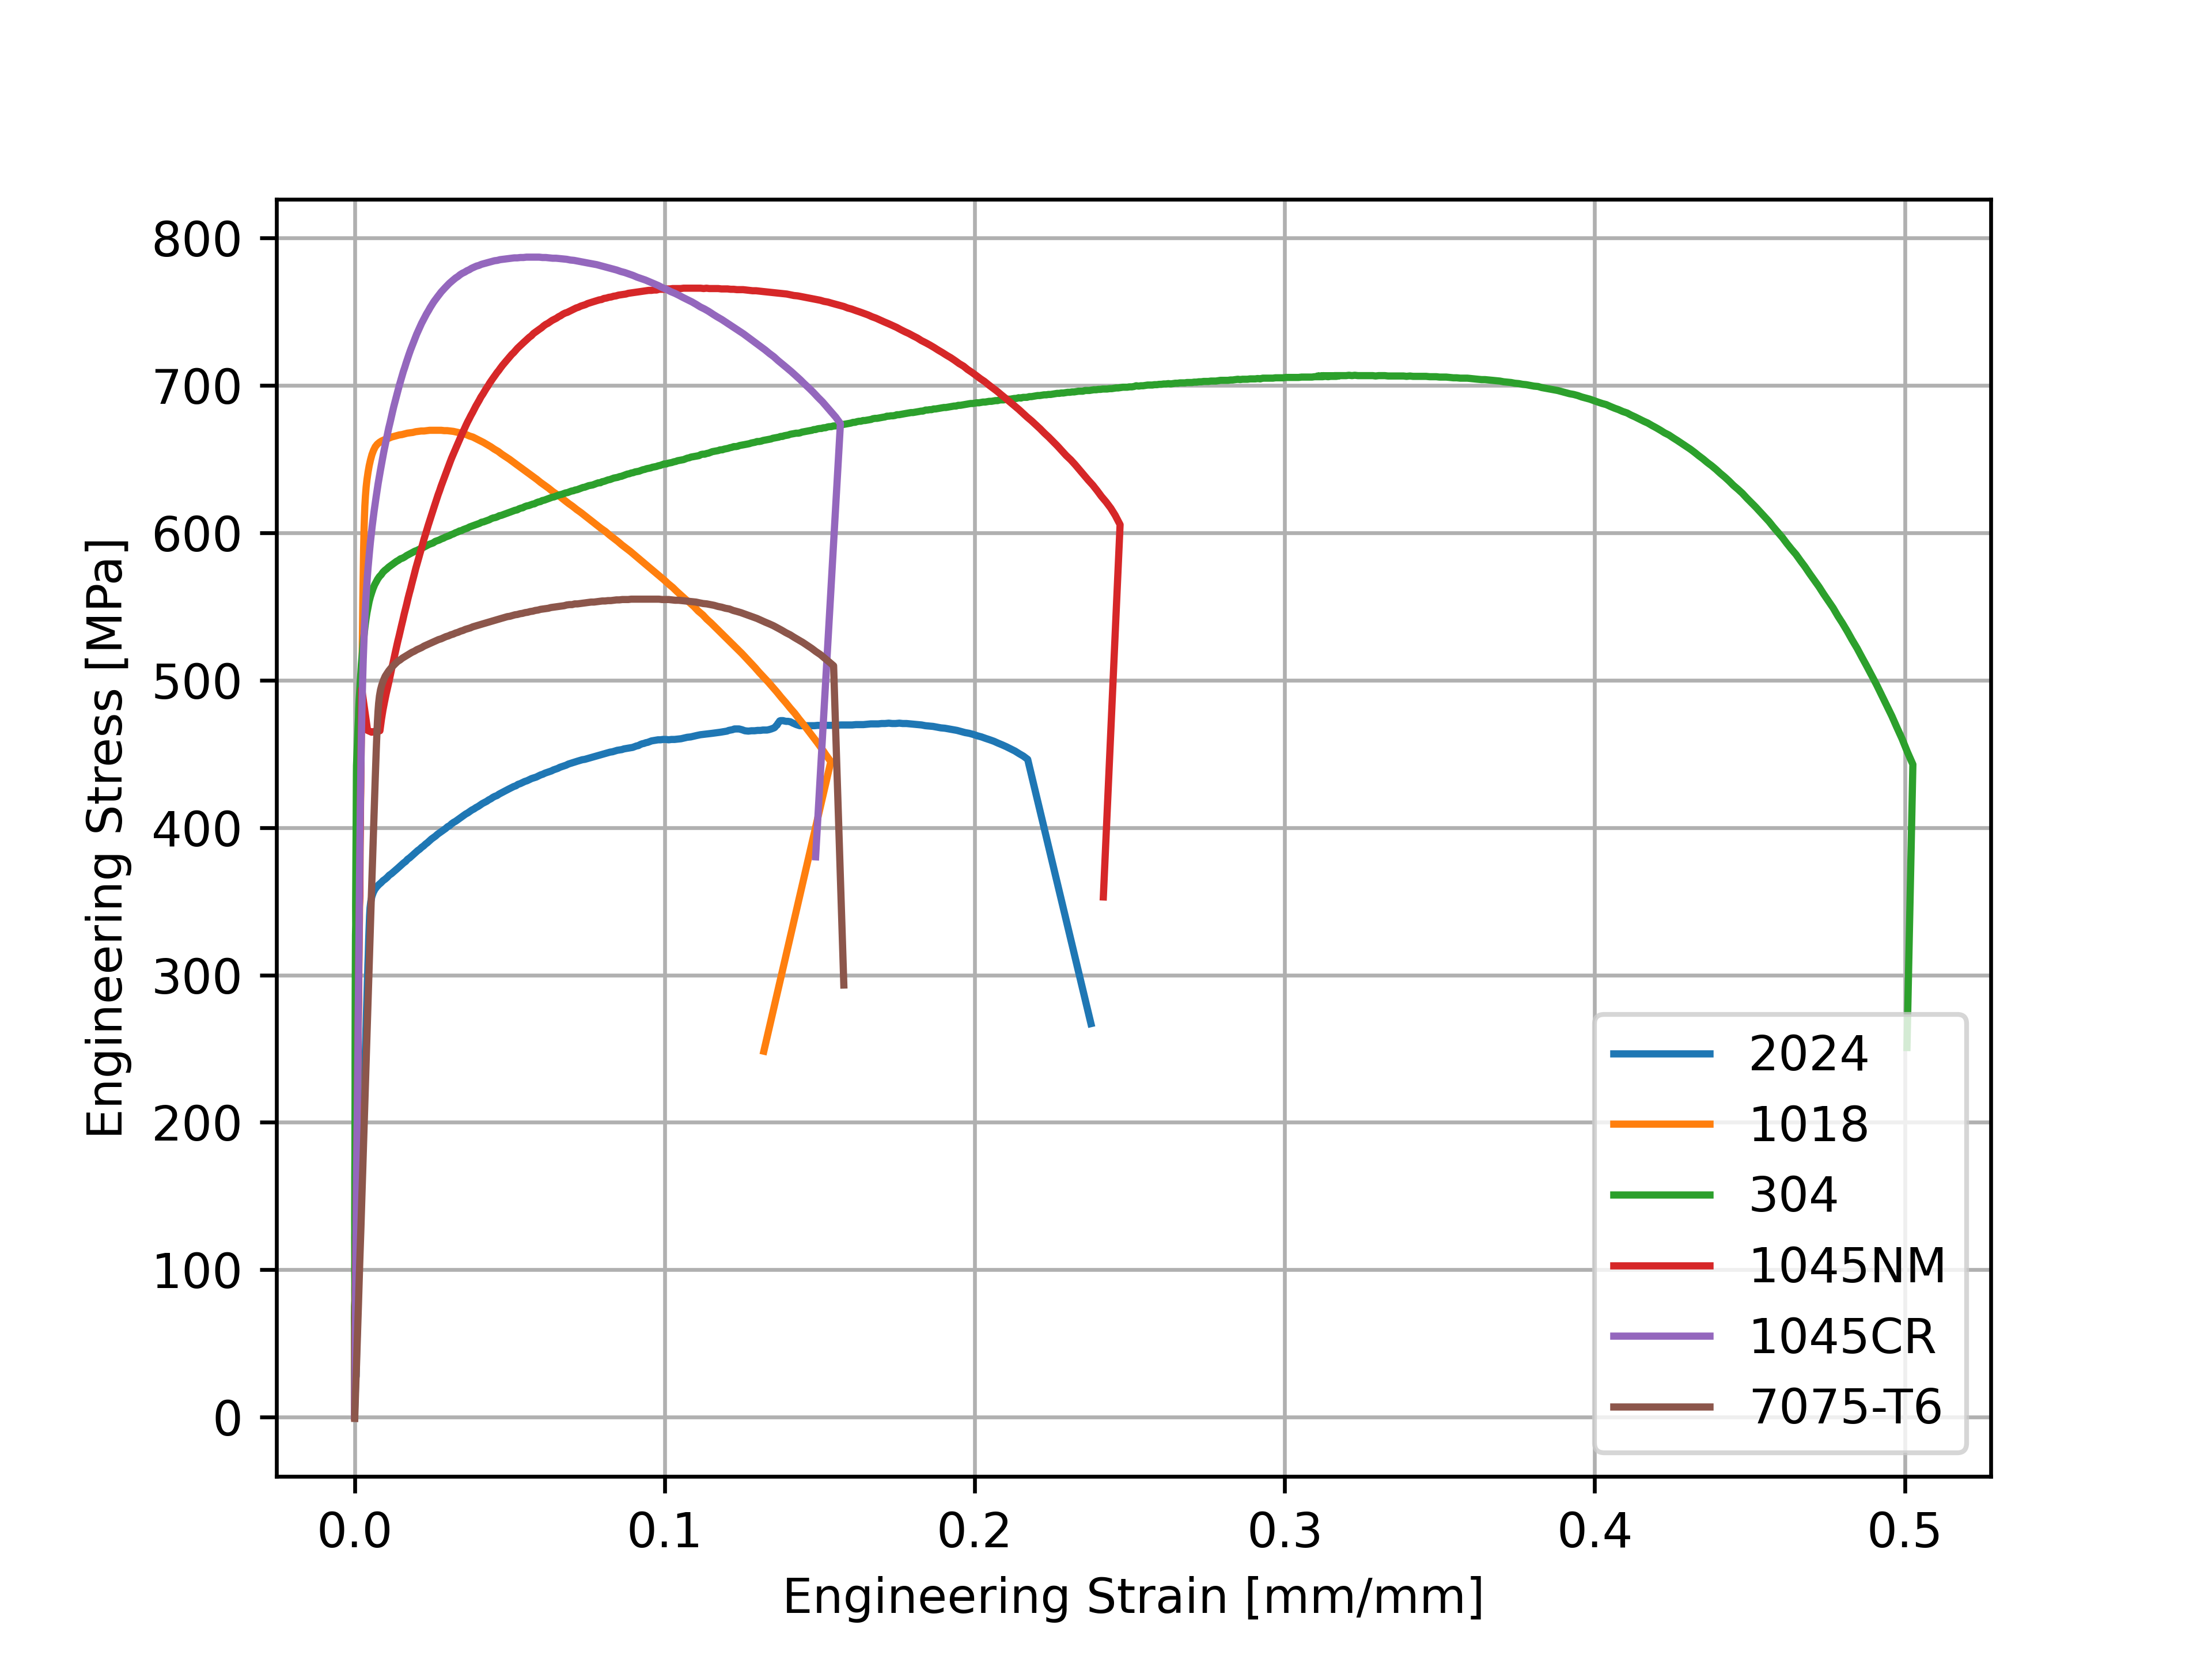
\includegraphics[width=0.5\linewidth]{plots/q1all.png}
    \caption{Caption}
    \label{fig:q1all}
\end{figure}

\begin{figure}[!h!]
    \centering
    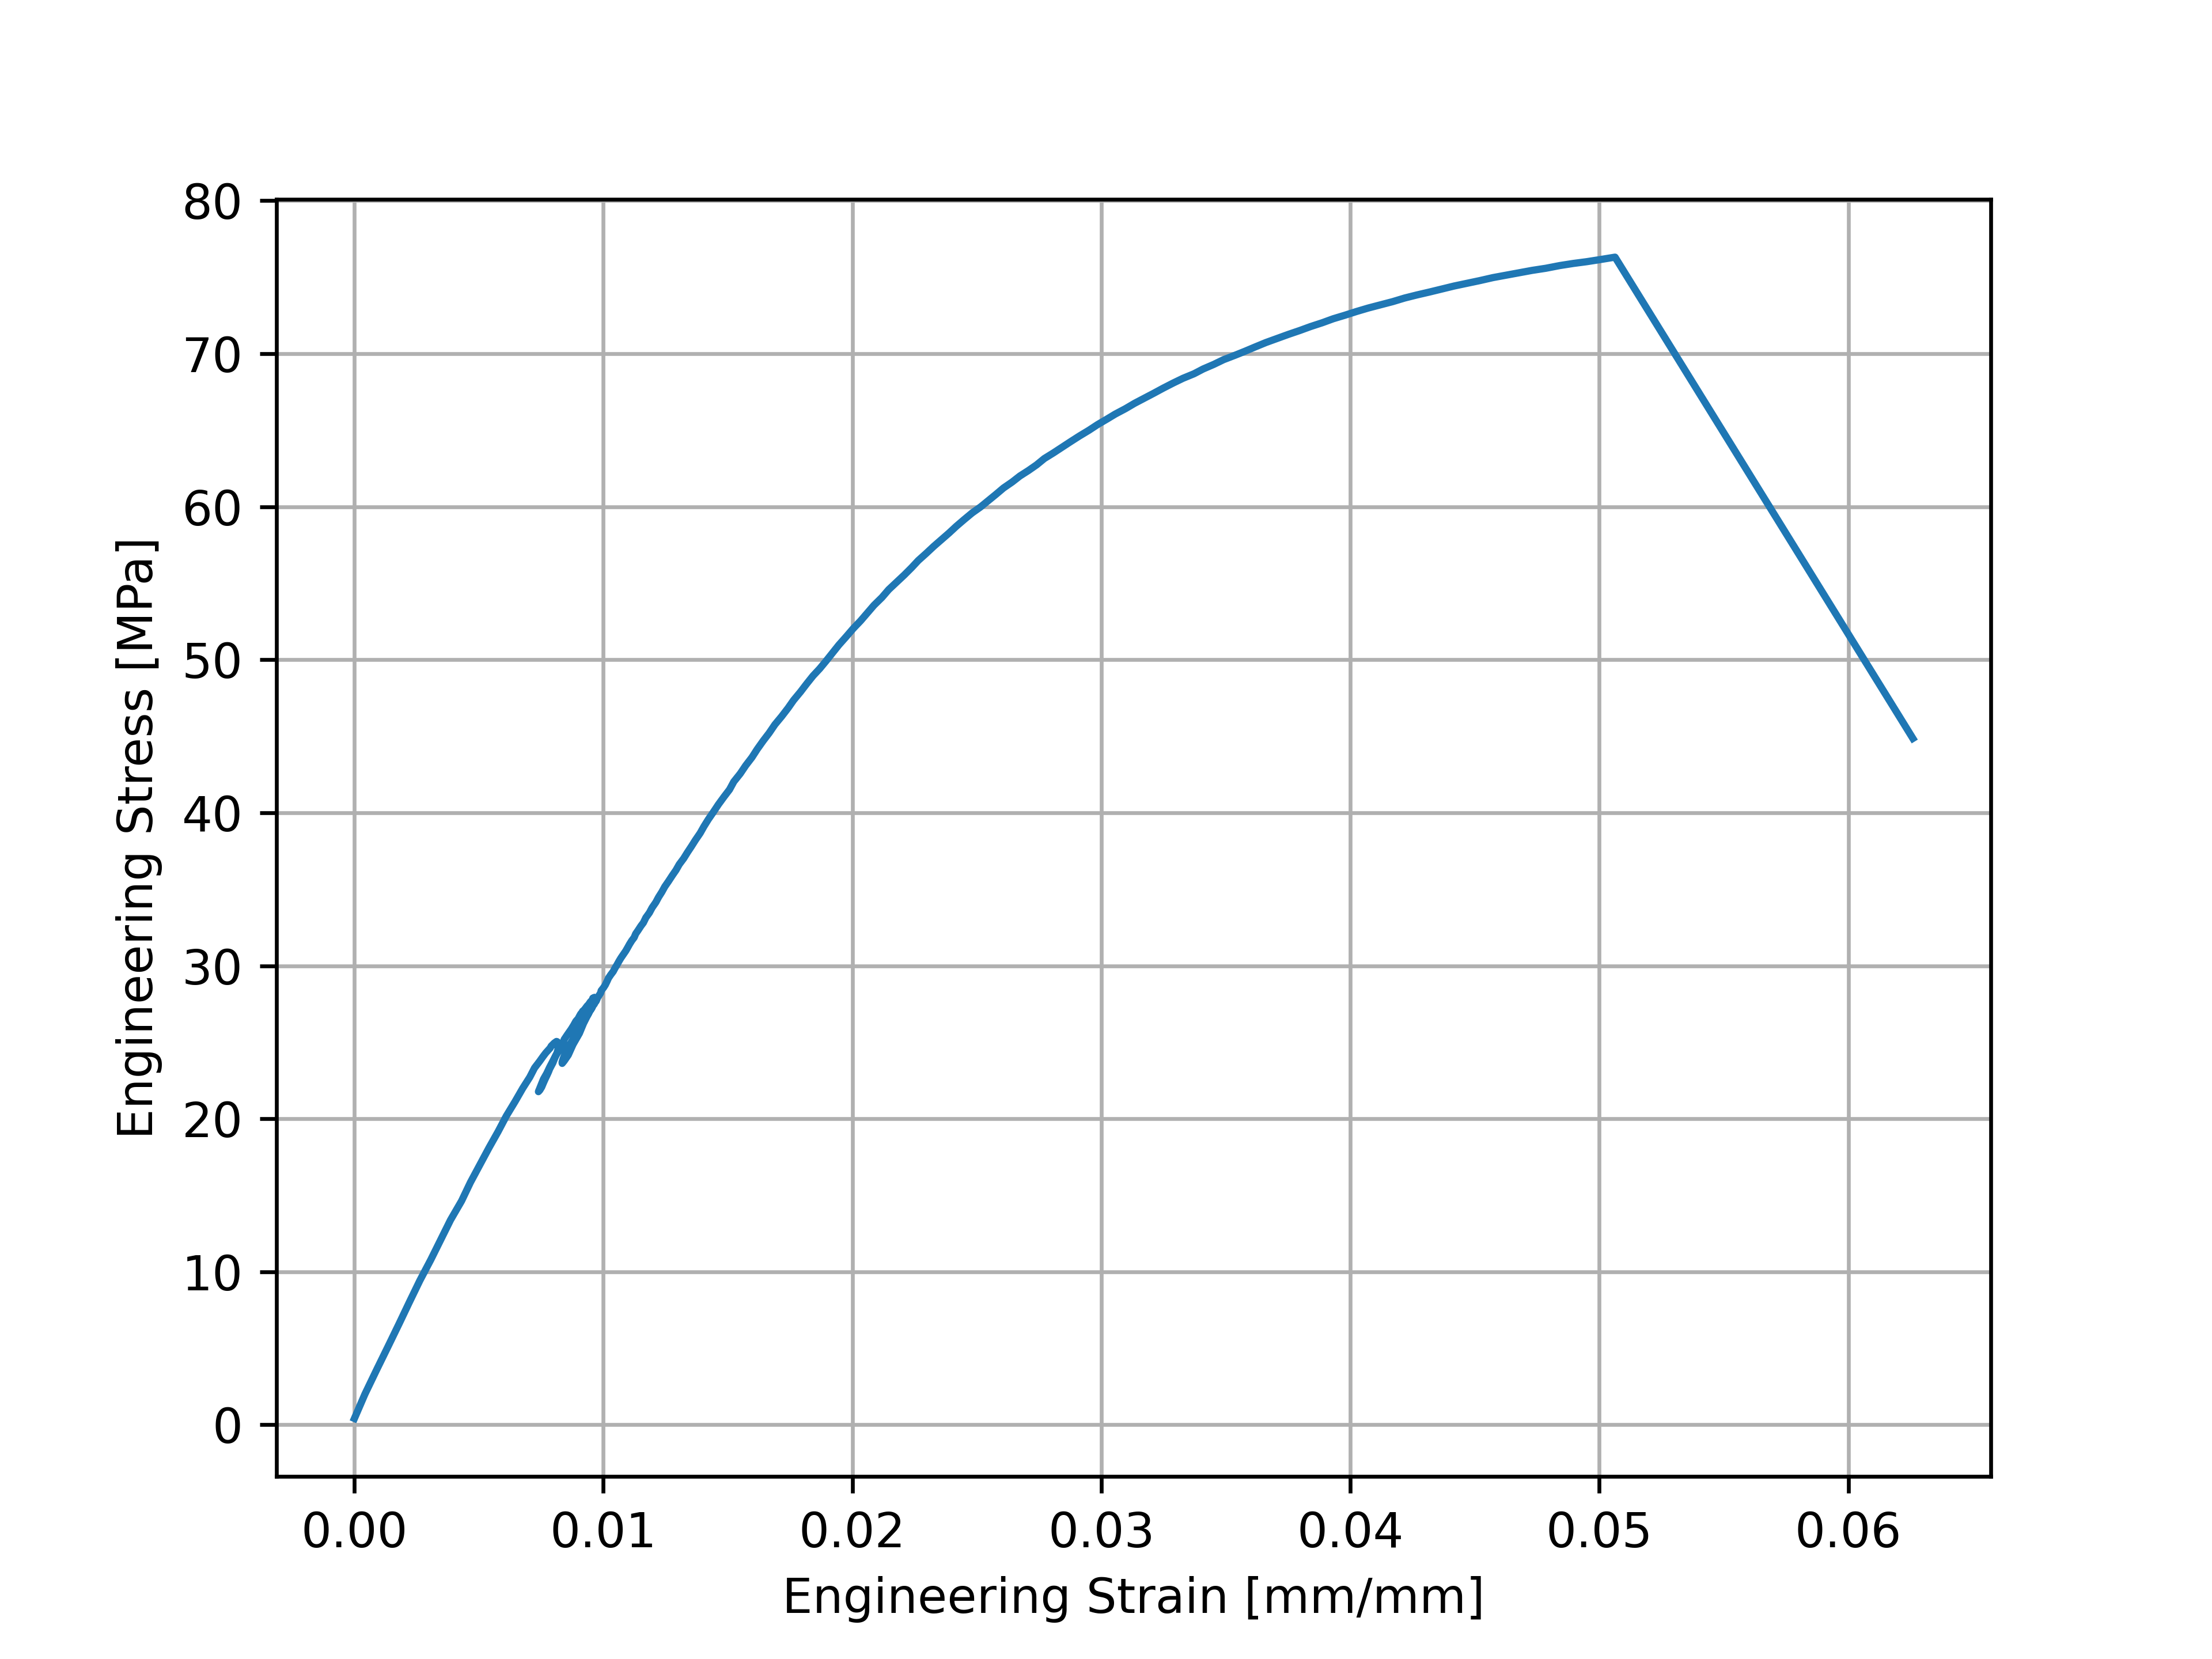
\includegraphics[width=0.5\linewidth]{plots/q1_PMMA.png}
    \caption{Caption}
    \label{fig:q1pmma}
\end{figure}

\subsection{Question 2}

\begin{table}[!h!]
    \centering
    \def\arraystretch{1.5}
    \caption{Tensile material properties for selected materials}
    \begin{tabular}{|c|c|c|c|c|c|}
         \toprule
         \hline
         \textbf{Material}& \textbf{2024} & \textbf{PMMA} & \textbf{1018} & \textbf{304} & \textbf{1045} \\
         \midrule
         \hline
         \textbf{Elastic Modulus [MPa]} & 71795.19 & 3150.347 & 204335.7 & 670381.1 & 203454.9 \\
         \textbf{Yield Strength [MPa]} & 359.4 & 42.7 & 649.8 & 525.3 & 465.8 \\
         \textbf{Ultimate Tensile Strength [MPa]} & 472.5526 & 76.31283 & 669.5332 & 706.8640 & 765.9465 \\
         \textbf{Percent Elongated} & 23.75166 & 6.258398 & 15.36075 & 50.26496 & 24.69000 \\
         \textbf{Modulus of Resilience} & 0.899561 & 0.289379 & 1.033201 & 0.205808 & 0.533213\\
         \textbf{Rockwell B Hardness} & 72.8 & N/A & 94.3 & 100.6 & 90.7 \\
         \hline
    \end{tabular}
    \label{tab:q2}
\end{table}


\subsection{Question 3}
\newpage

\begin{figure}[!h!] 
  \label{fig:q3} 
  \begin{minipage}[b]{0.5\linewidth}
    \centering
    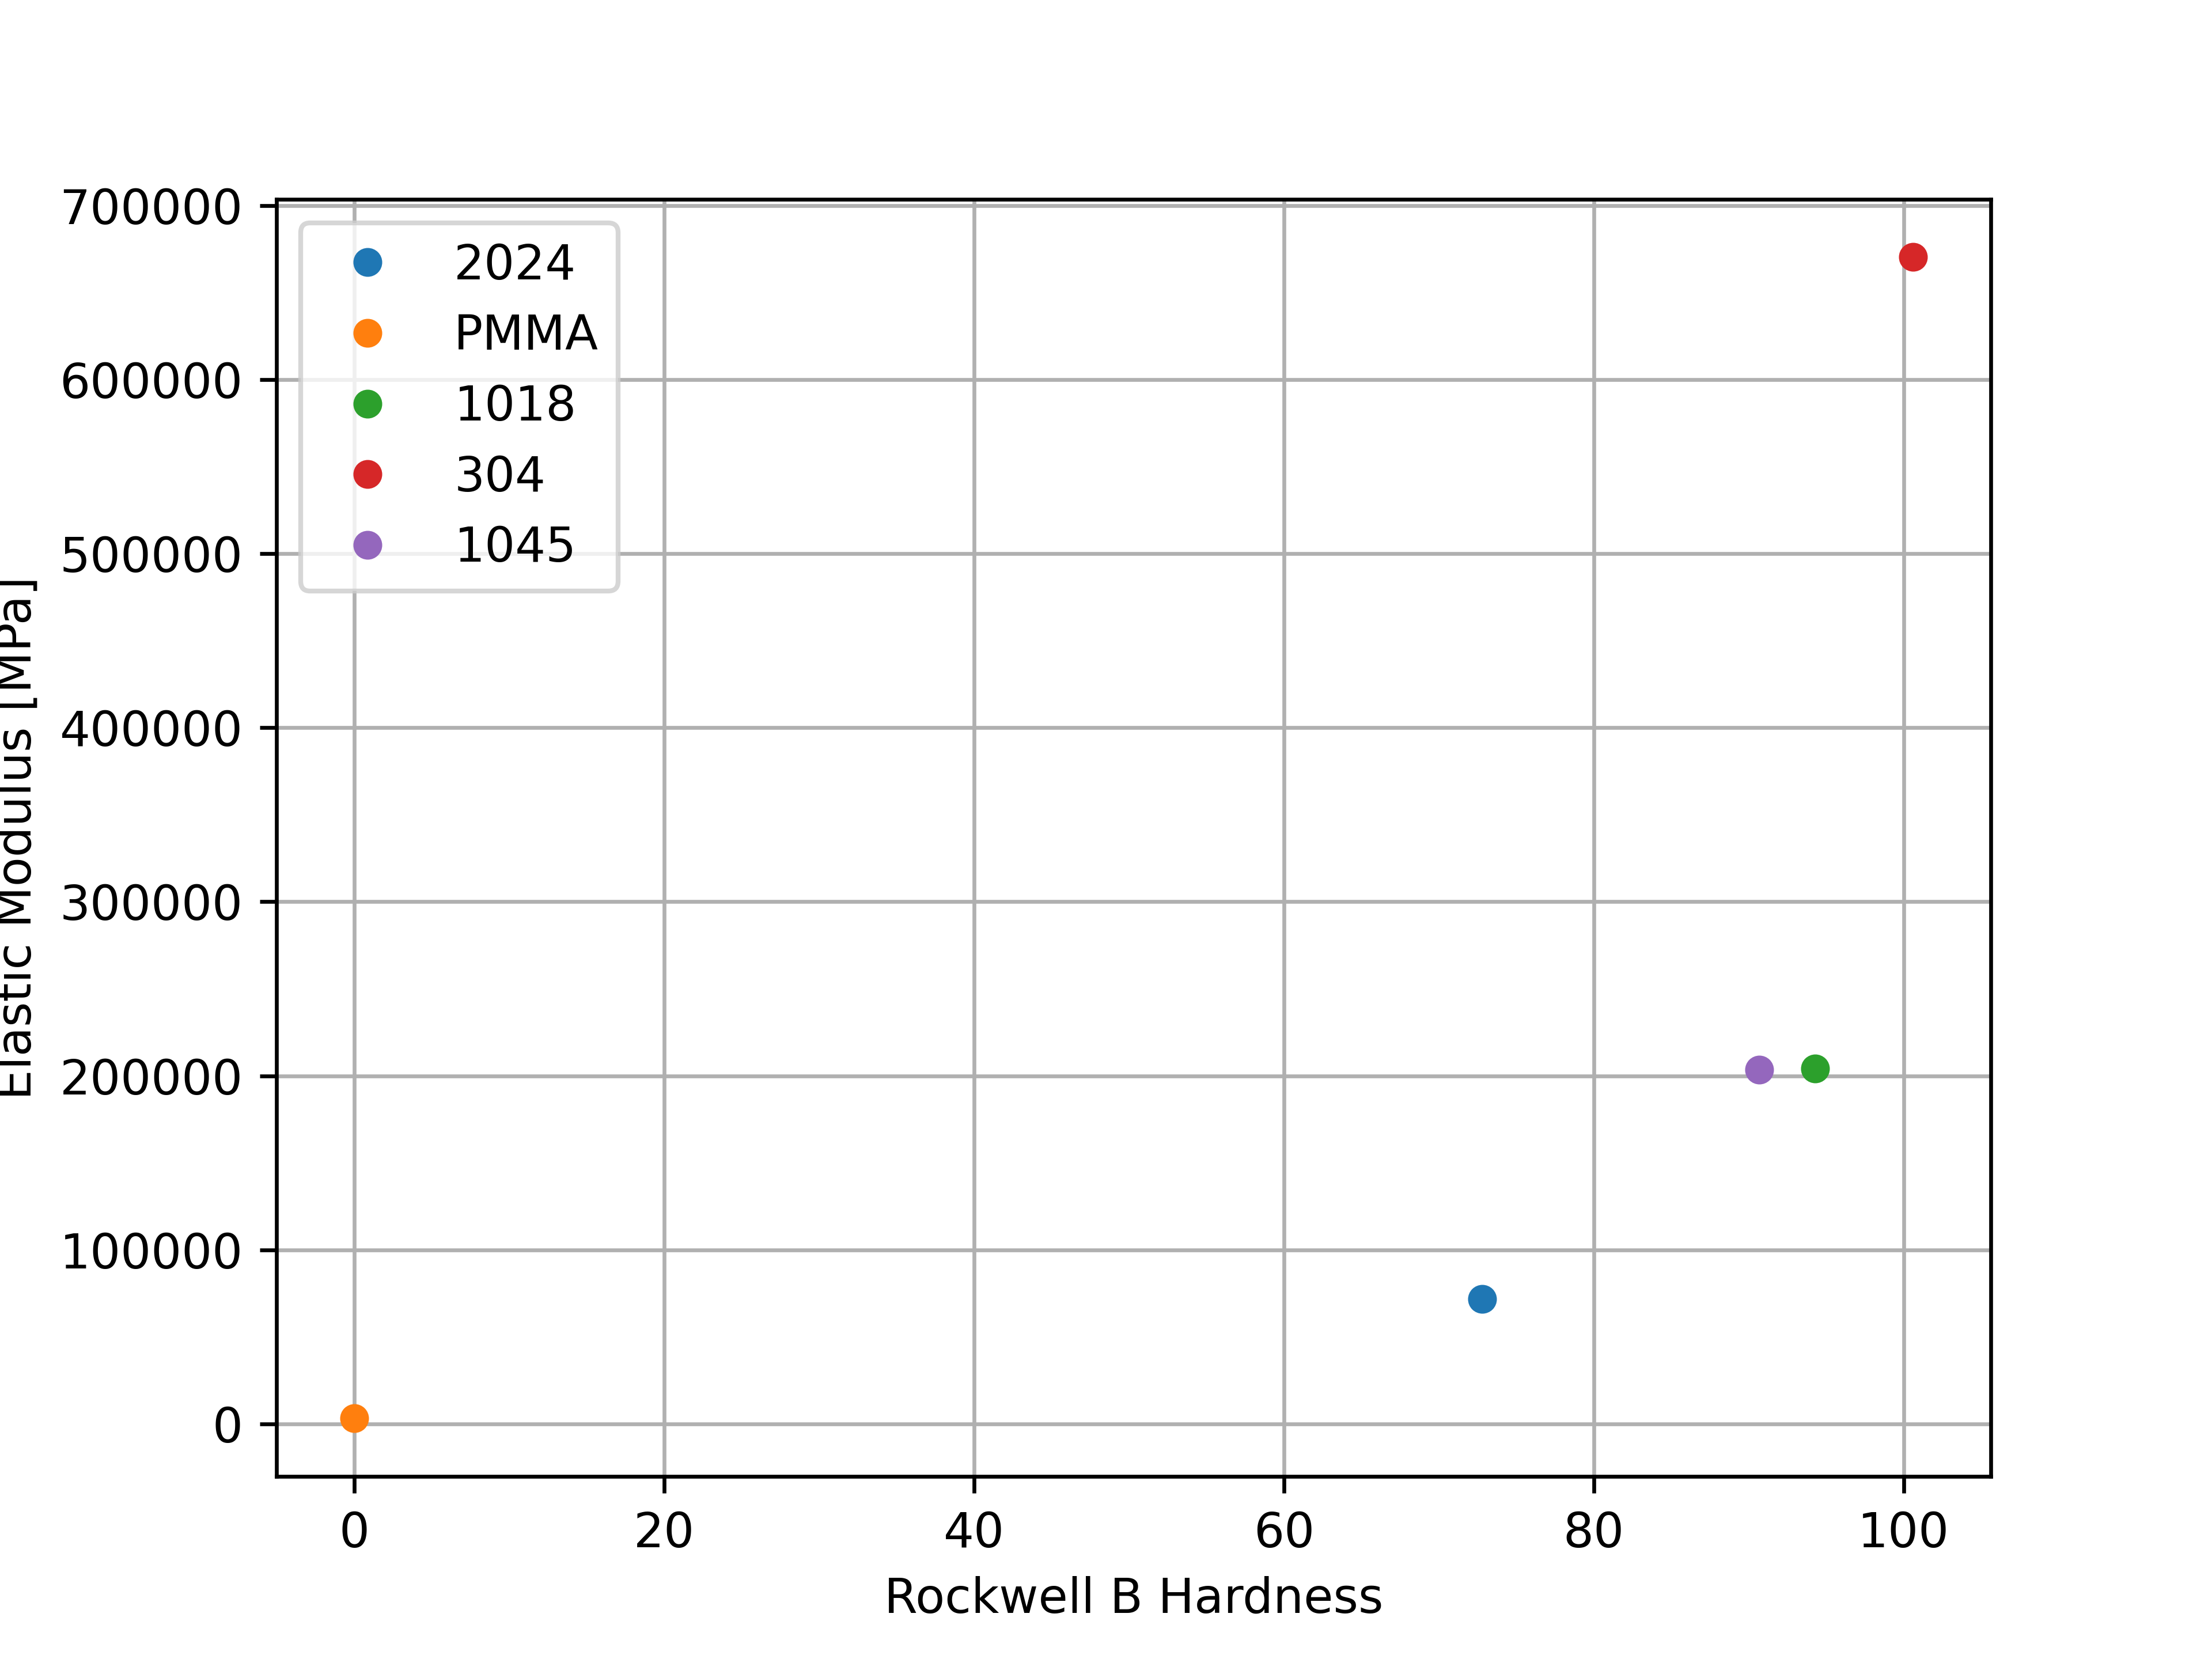
\includegraphics[width=\linewidth]{plots/q3_E.png} 
    \caption{Elastic Modulus as a function \\  of material hardness} 
    \vspace{4ex}
  \end{minipage}
  \begin{minipage}[b]{0.5\linewidth}
    \centering
    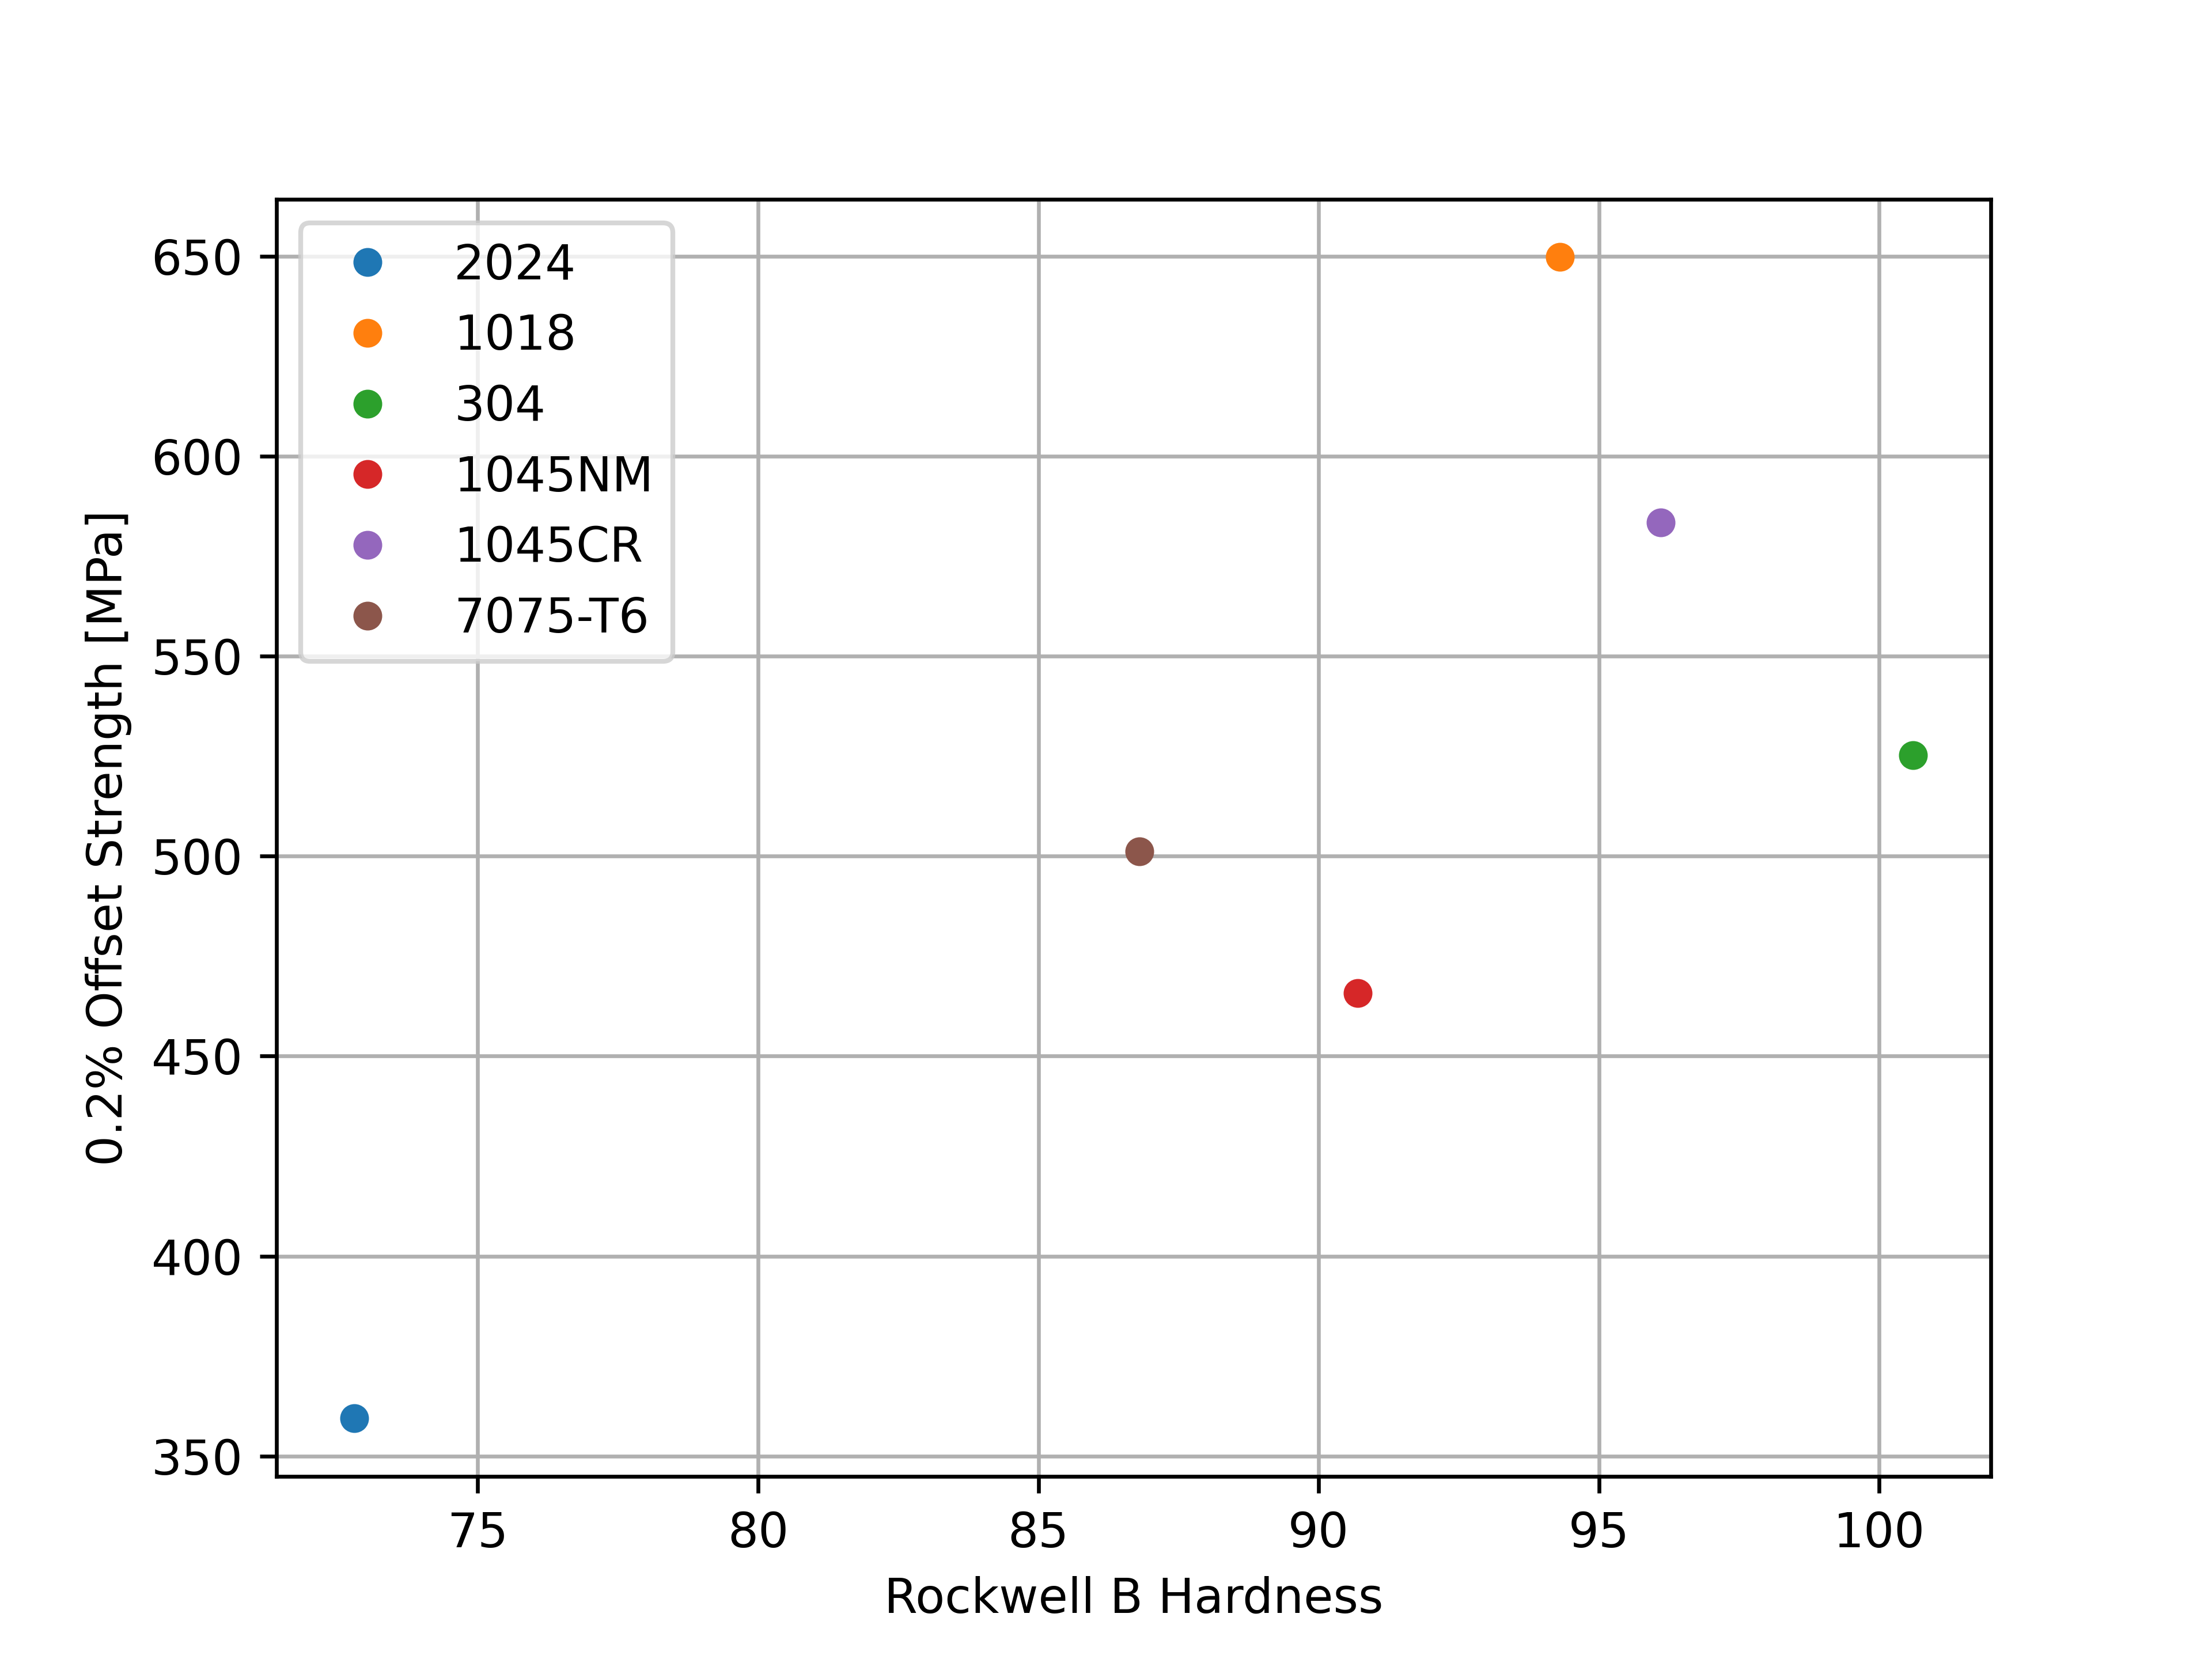
\includegraphics[width=\linewidth]{plots/q3_offstr.png} 
    \caption{Yield Strength as a function \\ of material hardness} 
    \vspace{4ex}
  \end{minipage} 
  \begin{minipage}[b]{0.5\linewidth}
    \centering
    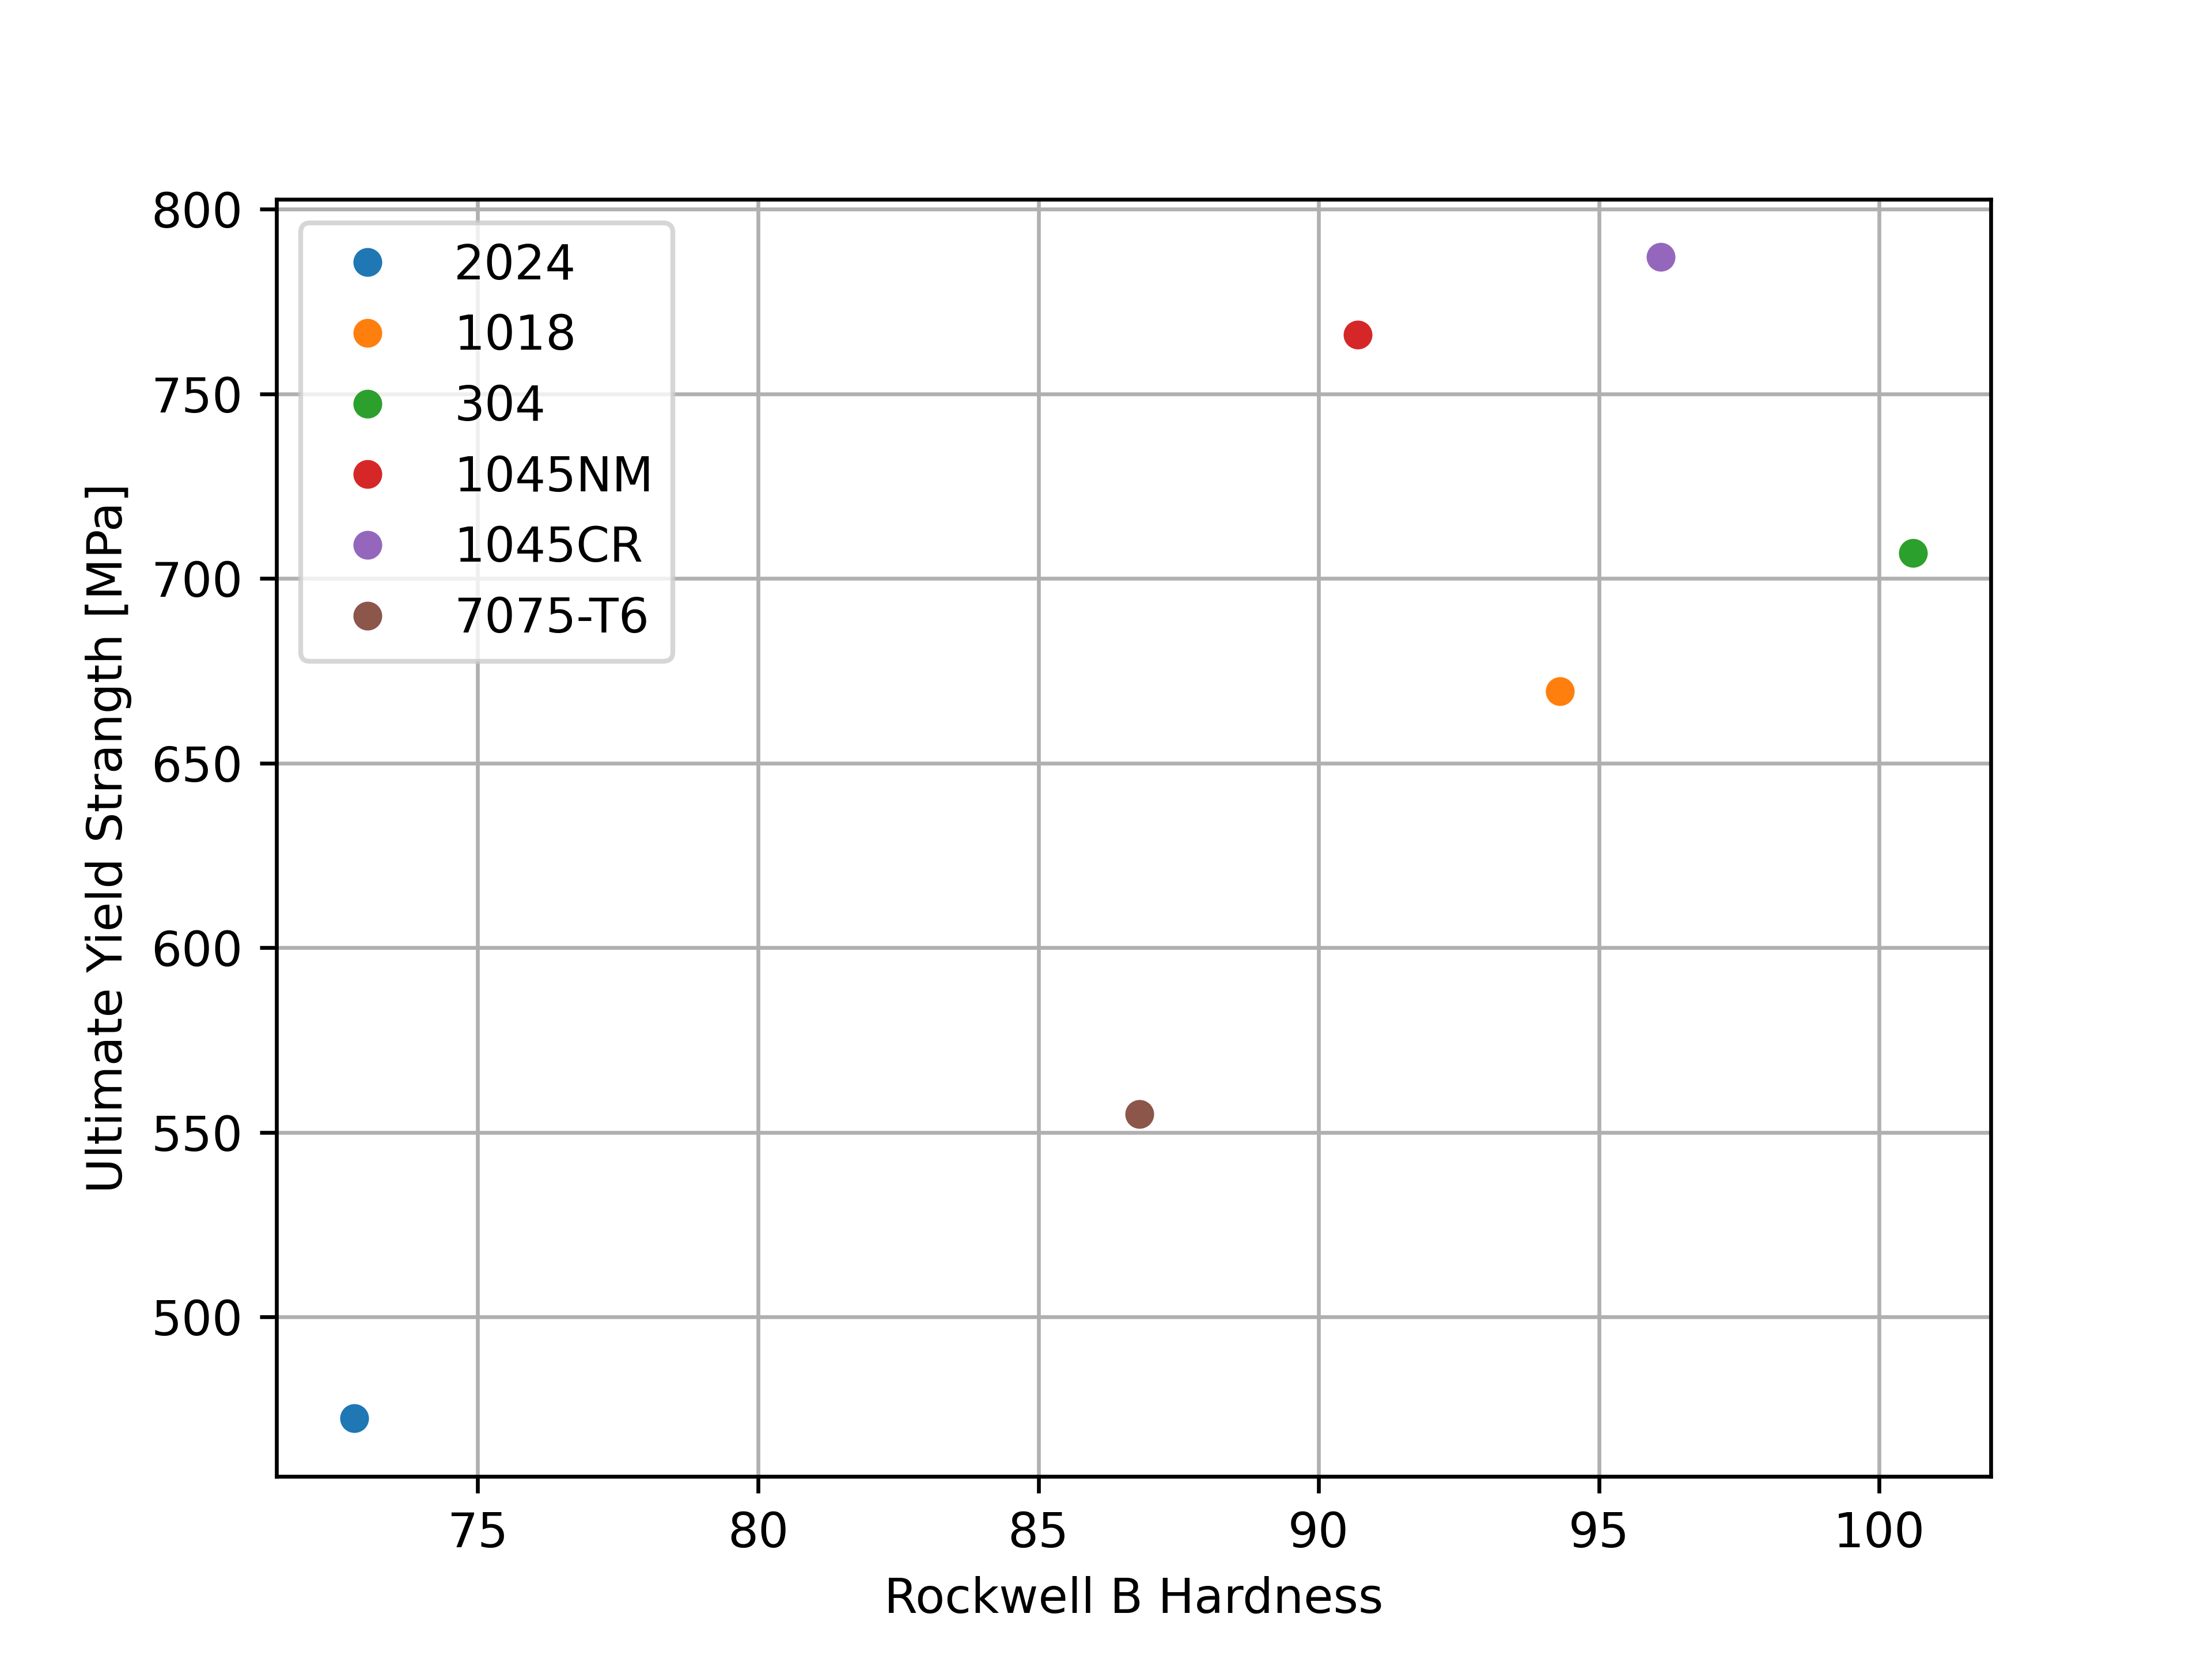
\includegraphics[width=\linewidth]{plots/q3_uts.png} 
    \caption{Ultimate Tensile Strength as a \\ function of material hardness} 
    \vspace{4ex}
  \end{minipage}
  \begin{minipage}[b]{0.5\linewidth}
    \centering
    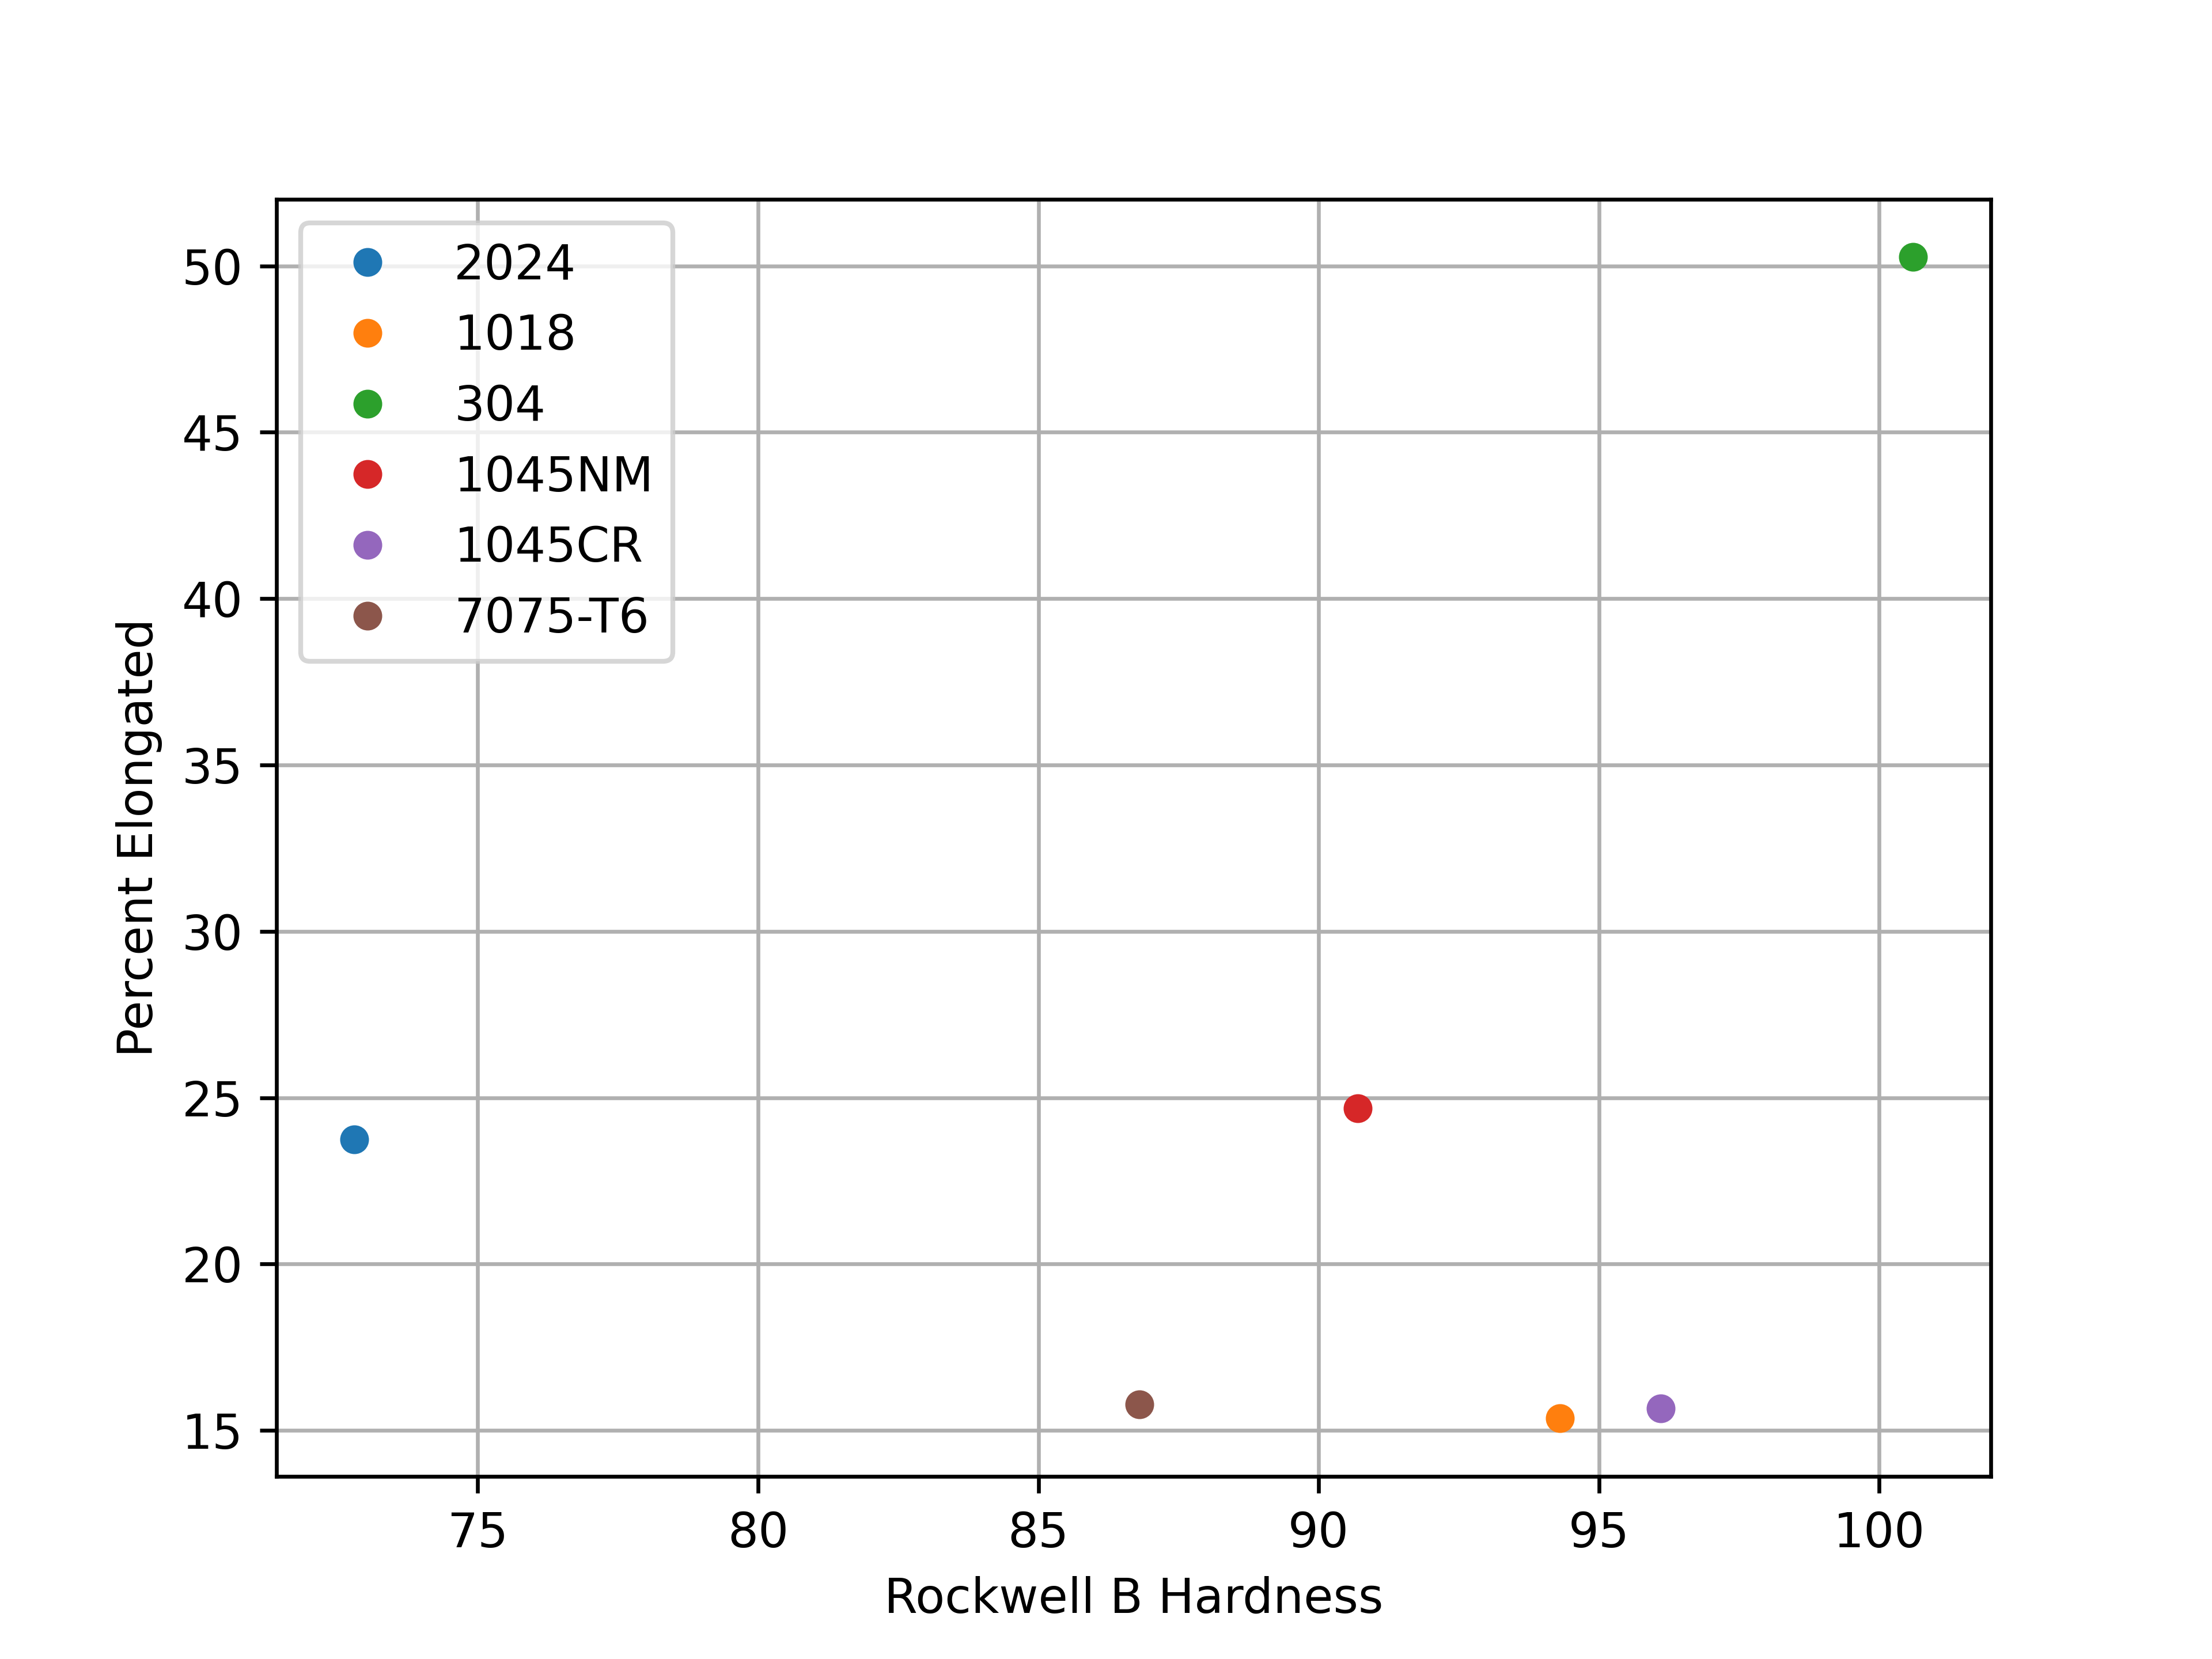
\includegraphics[width=\linewidth]{plots/q3_perelong.png} 
    \caption{Percent Elongation as a function \\ of material hardness} 
    \vspace{4ex}
  \end{minipage} 
  \begin{minipage}[b]{\linewidth}
      \centering
      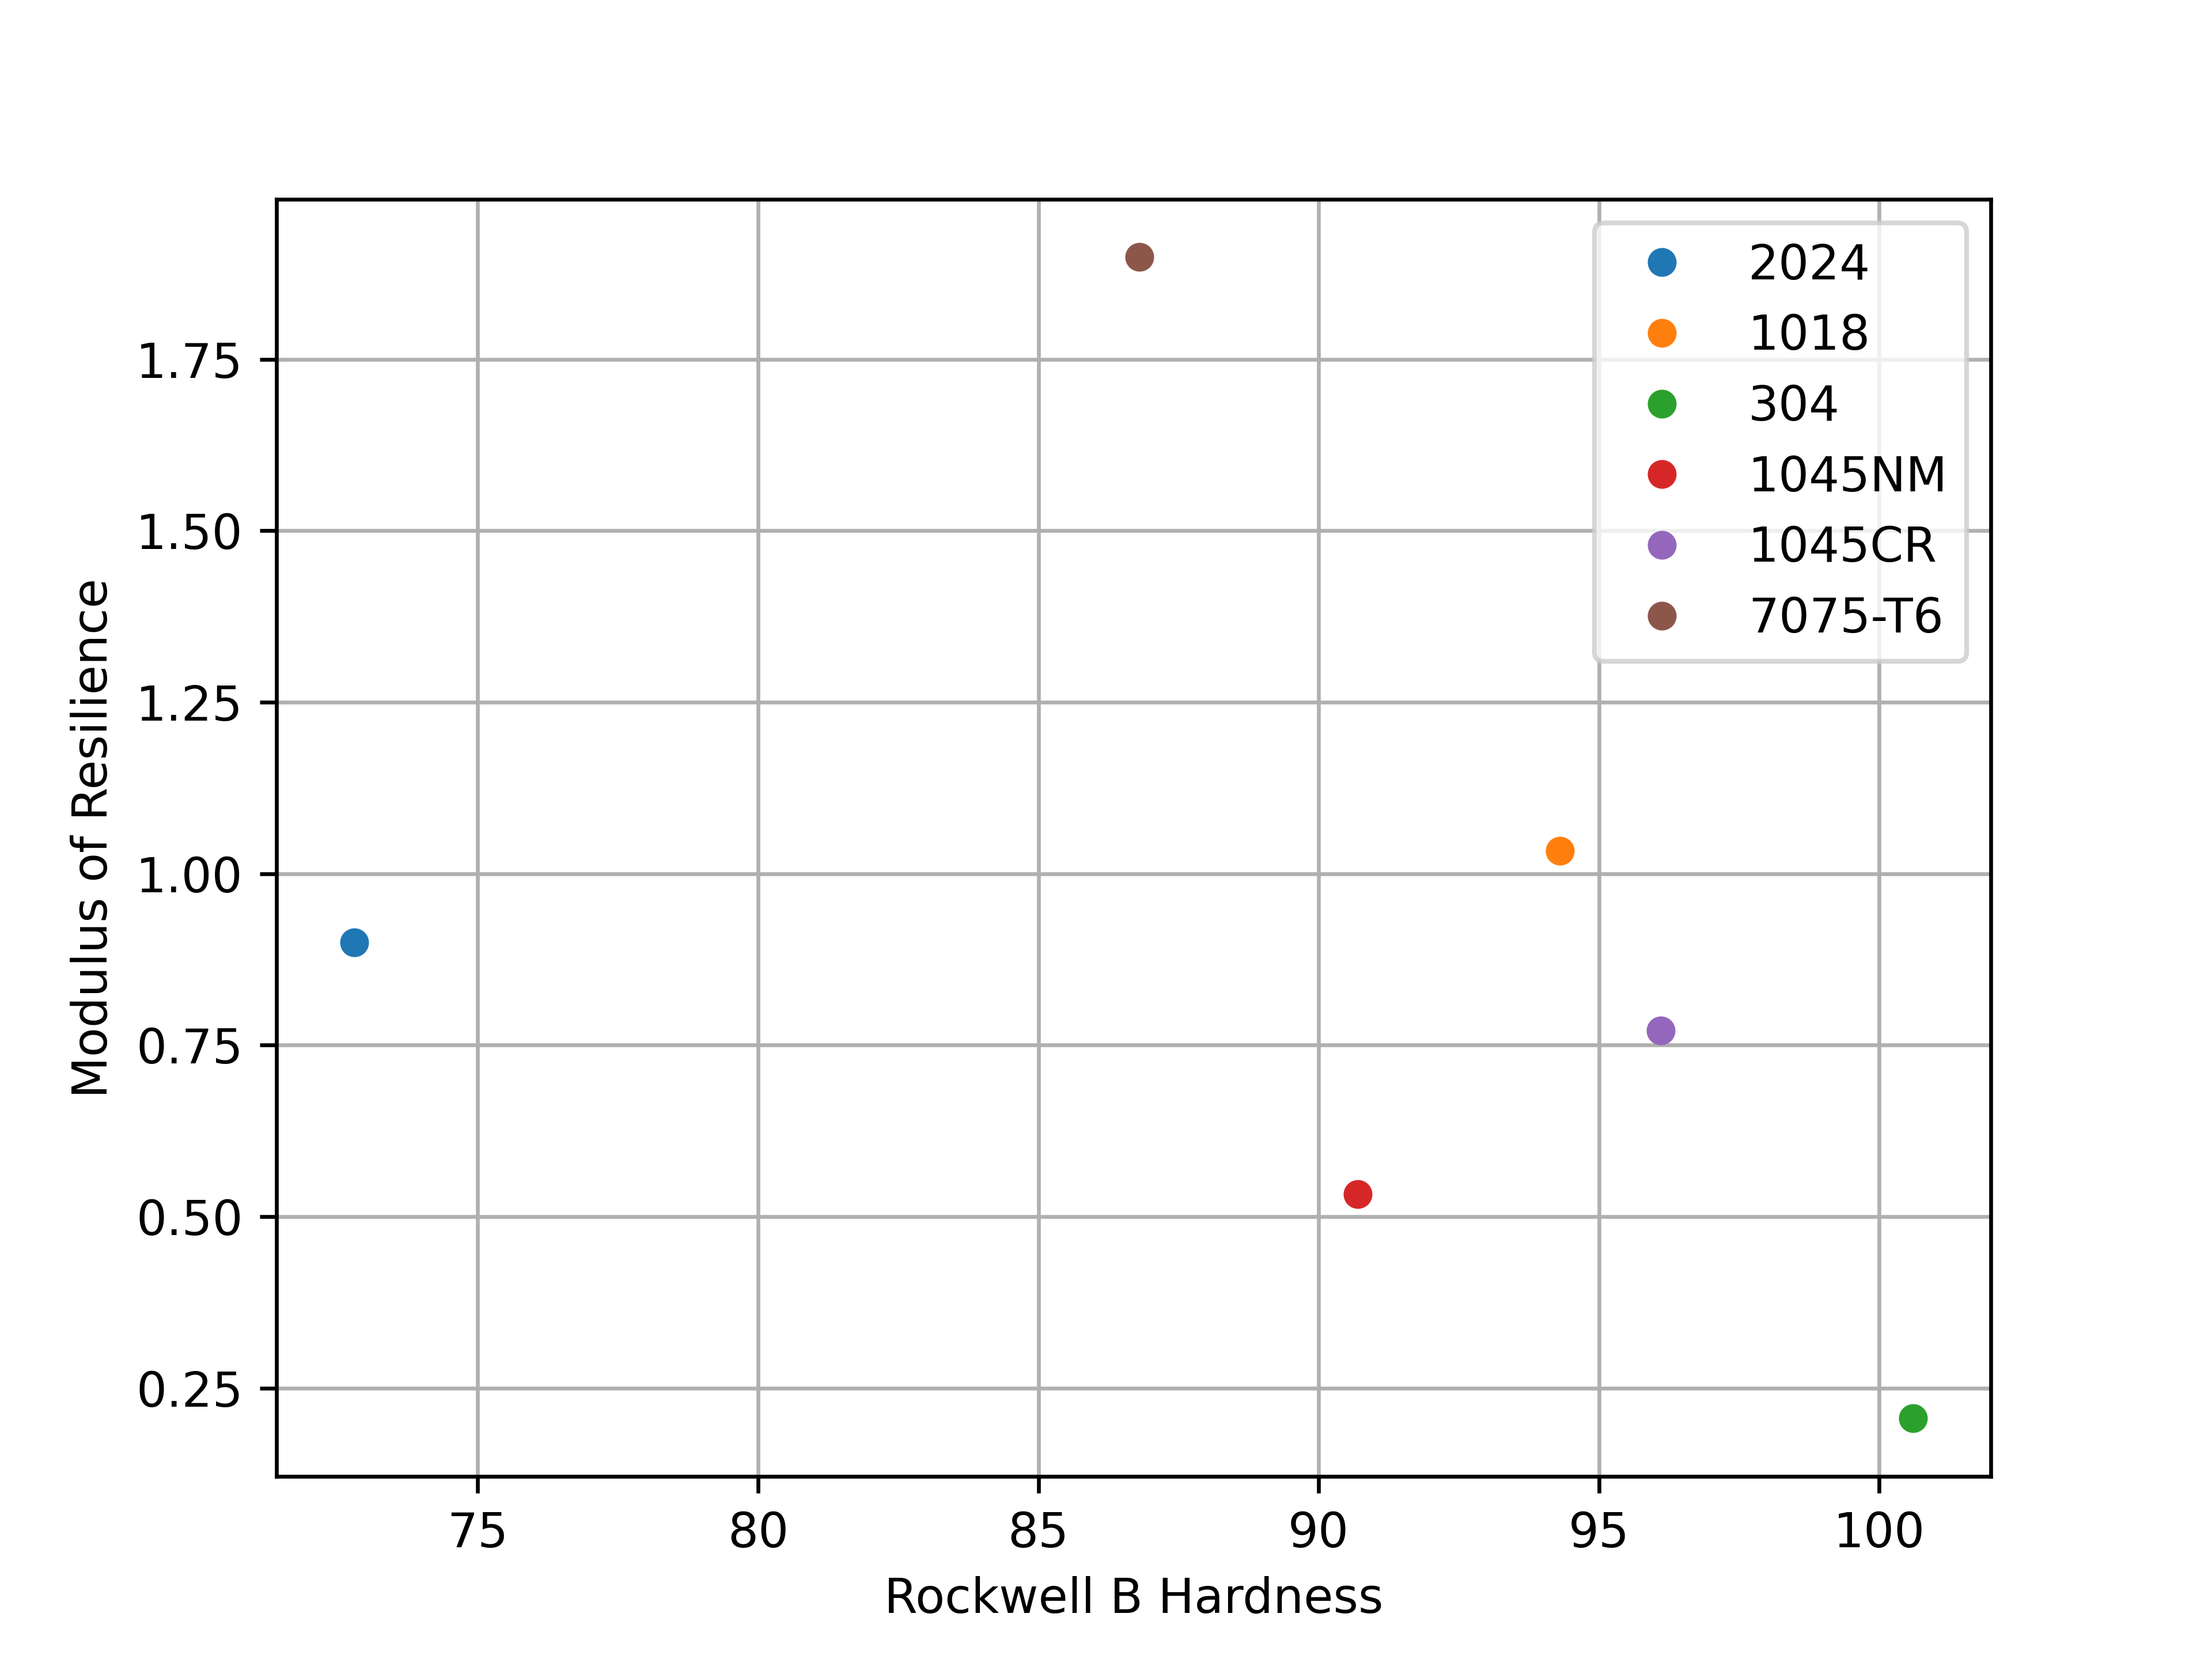
\includegraphics[width = .5\linewidth]{plots/q3_resilmod.png}
      \caption{Modulus of Resilience as a function of material hardness}
  \end{minipage}
\end{figure}
\newpage

\subsection{Question 4}
\begin{figure}
    \centering
    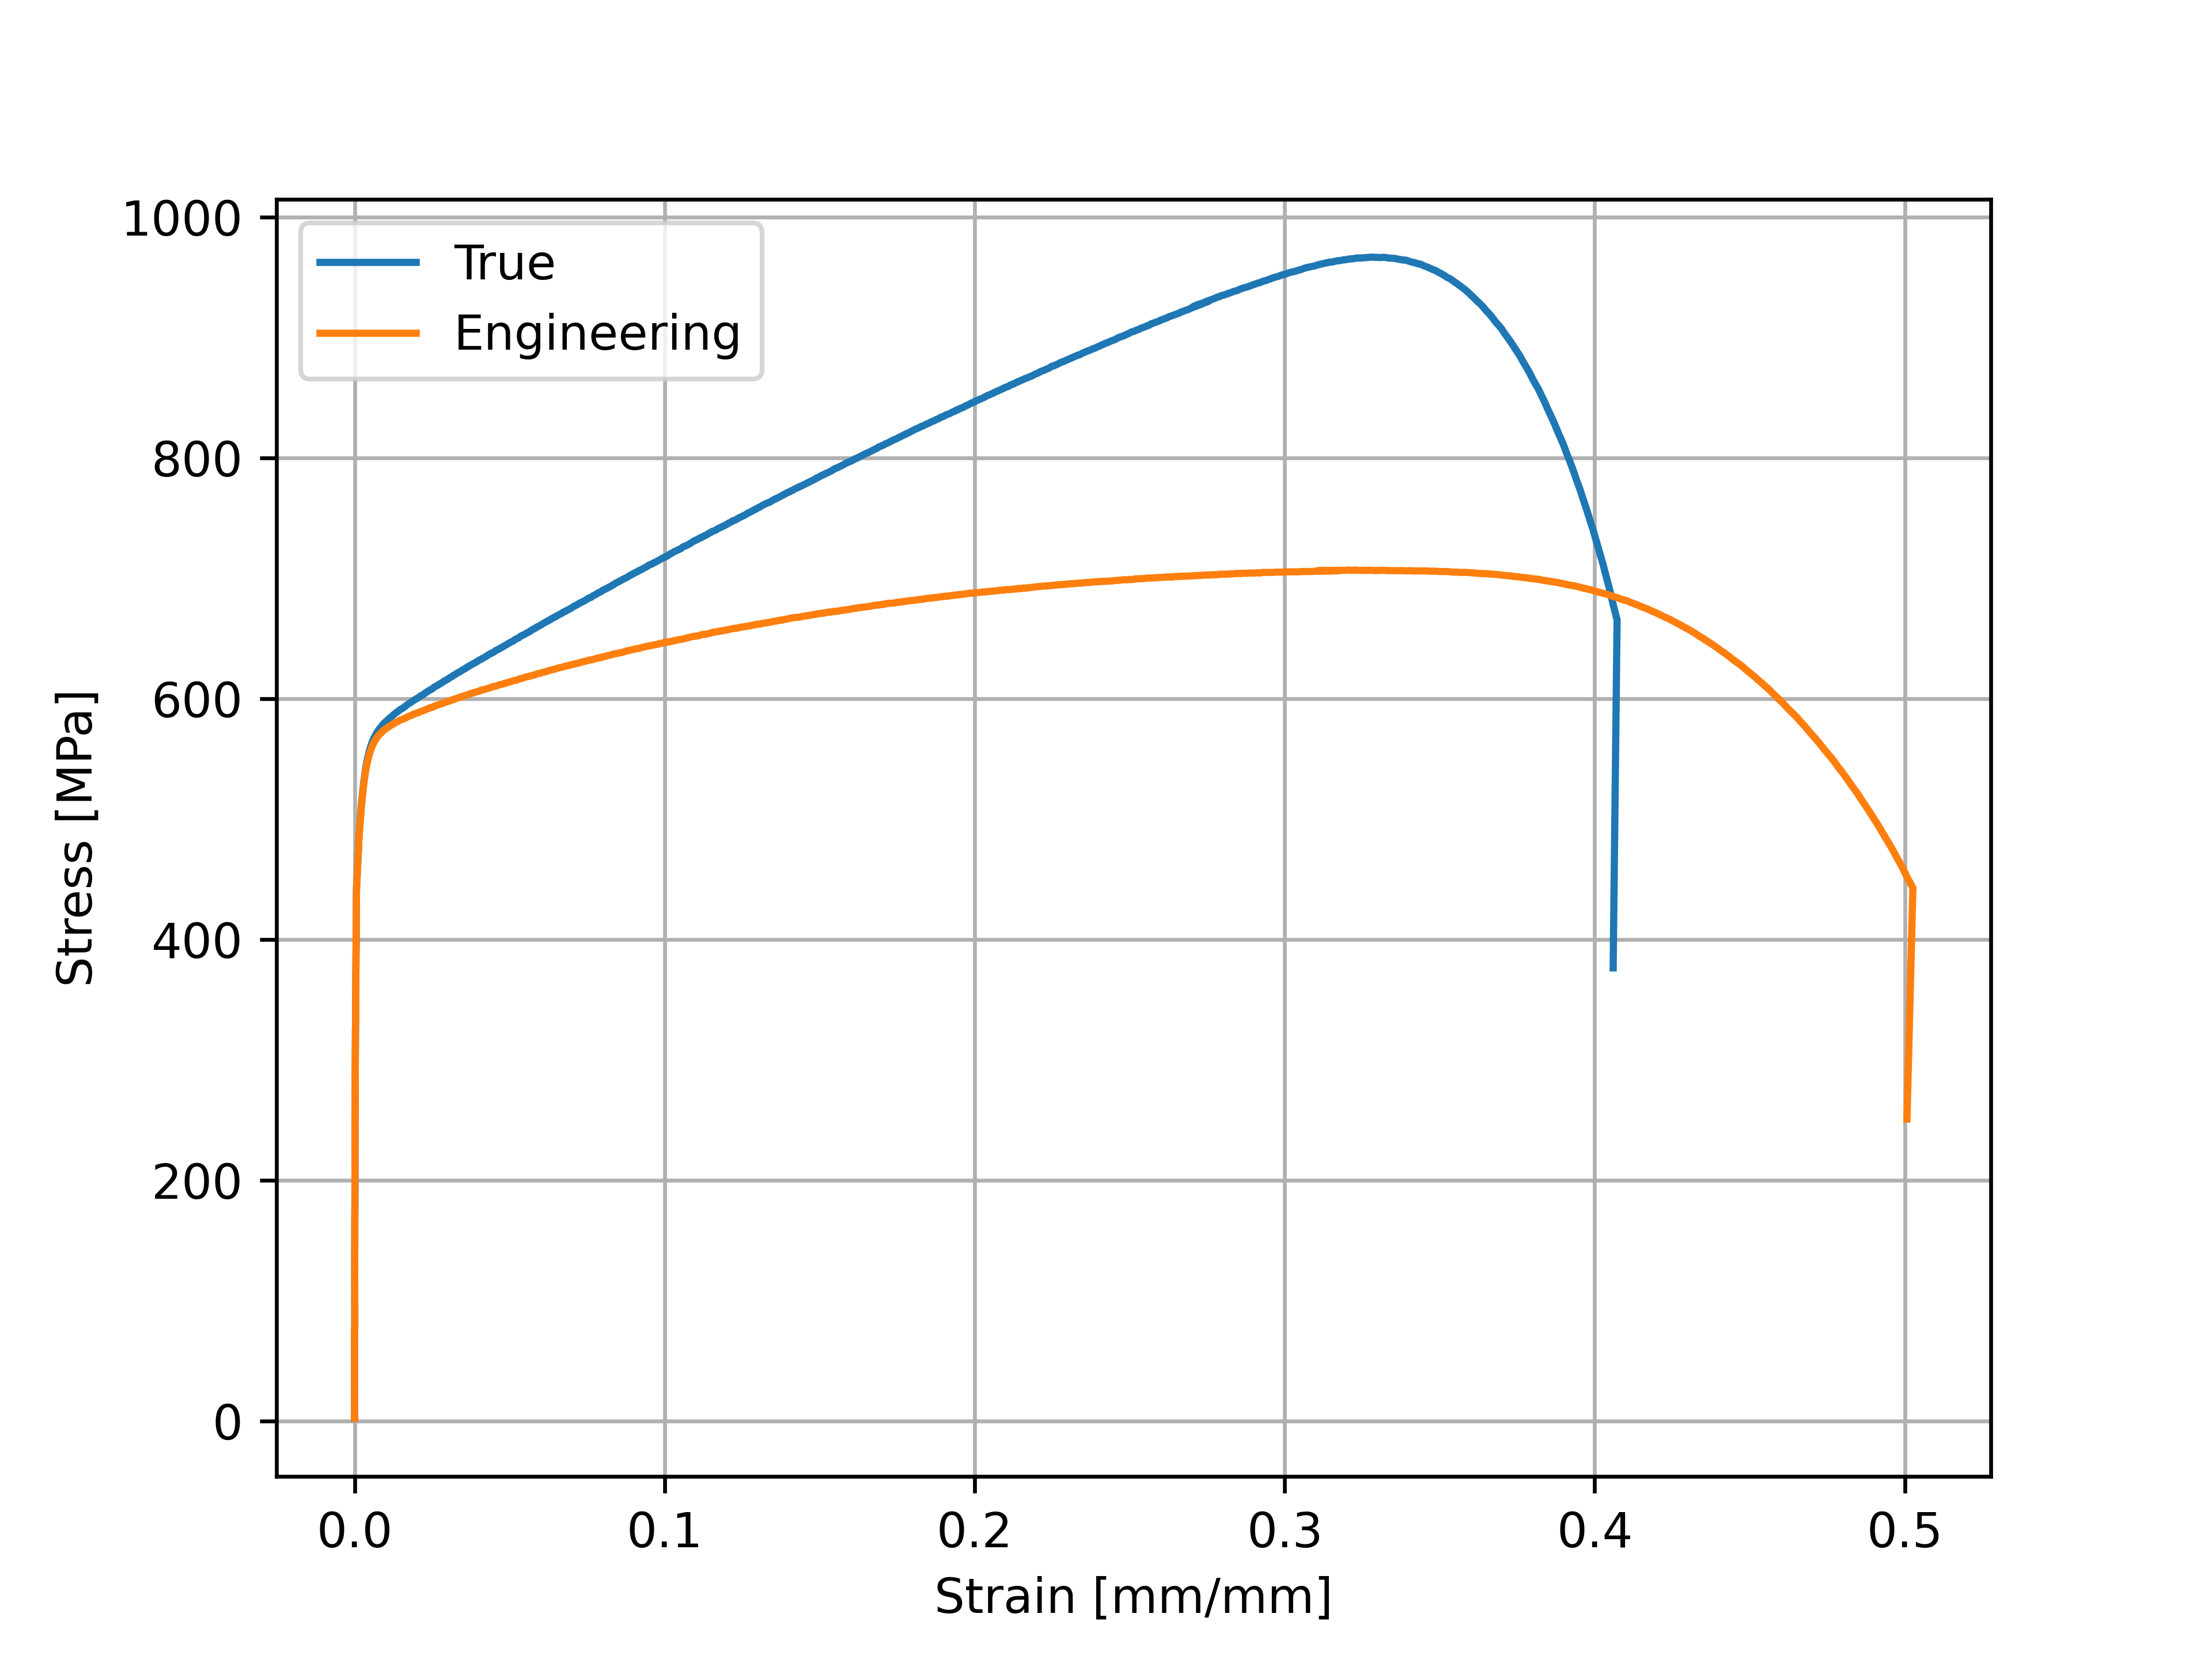
\includegraphics[width=0.5\linewidth]{plots/q4_evt.png}
    \caption{304 Stainless Steel engineering and true stress-strain}
    \label{fig:q4evt}
\end{figure}

\subsection{Question 5}
\begin{figure}
    \centering
    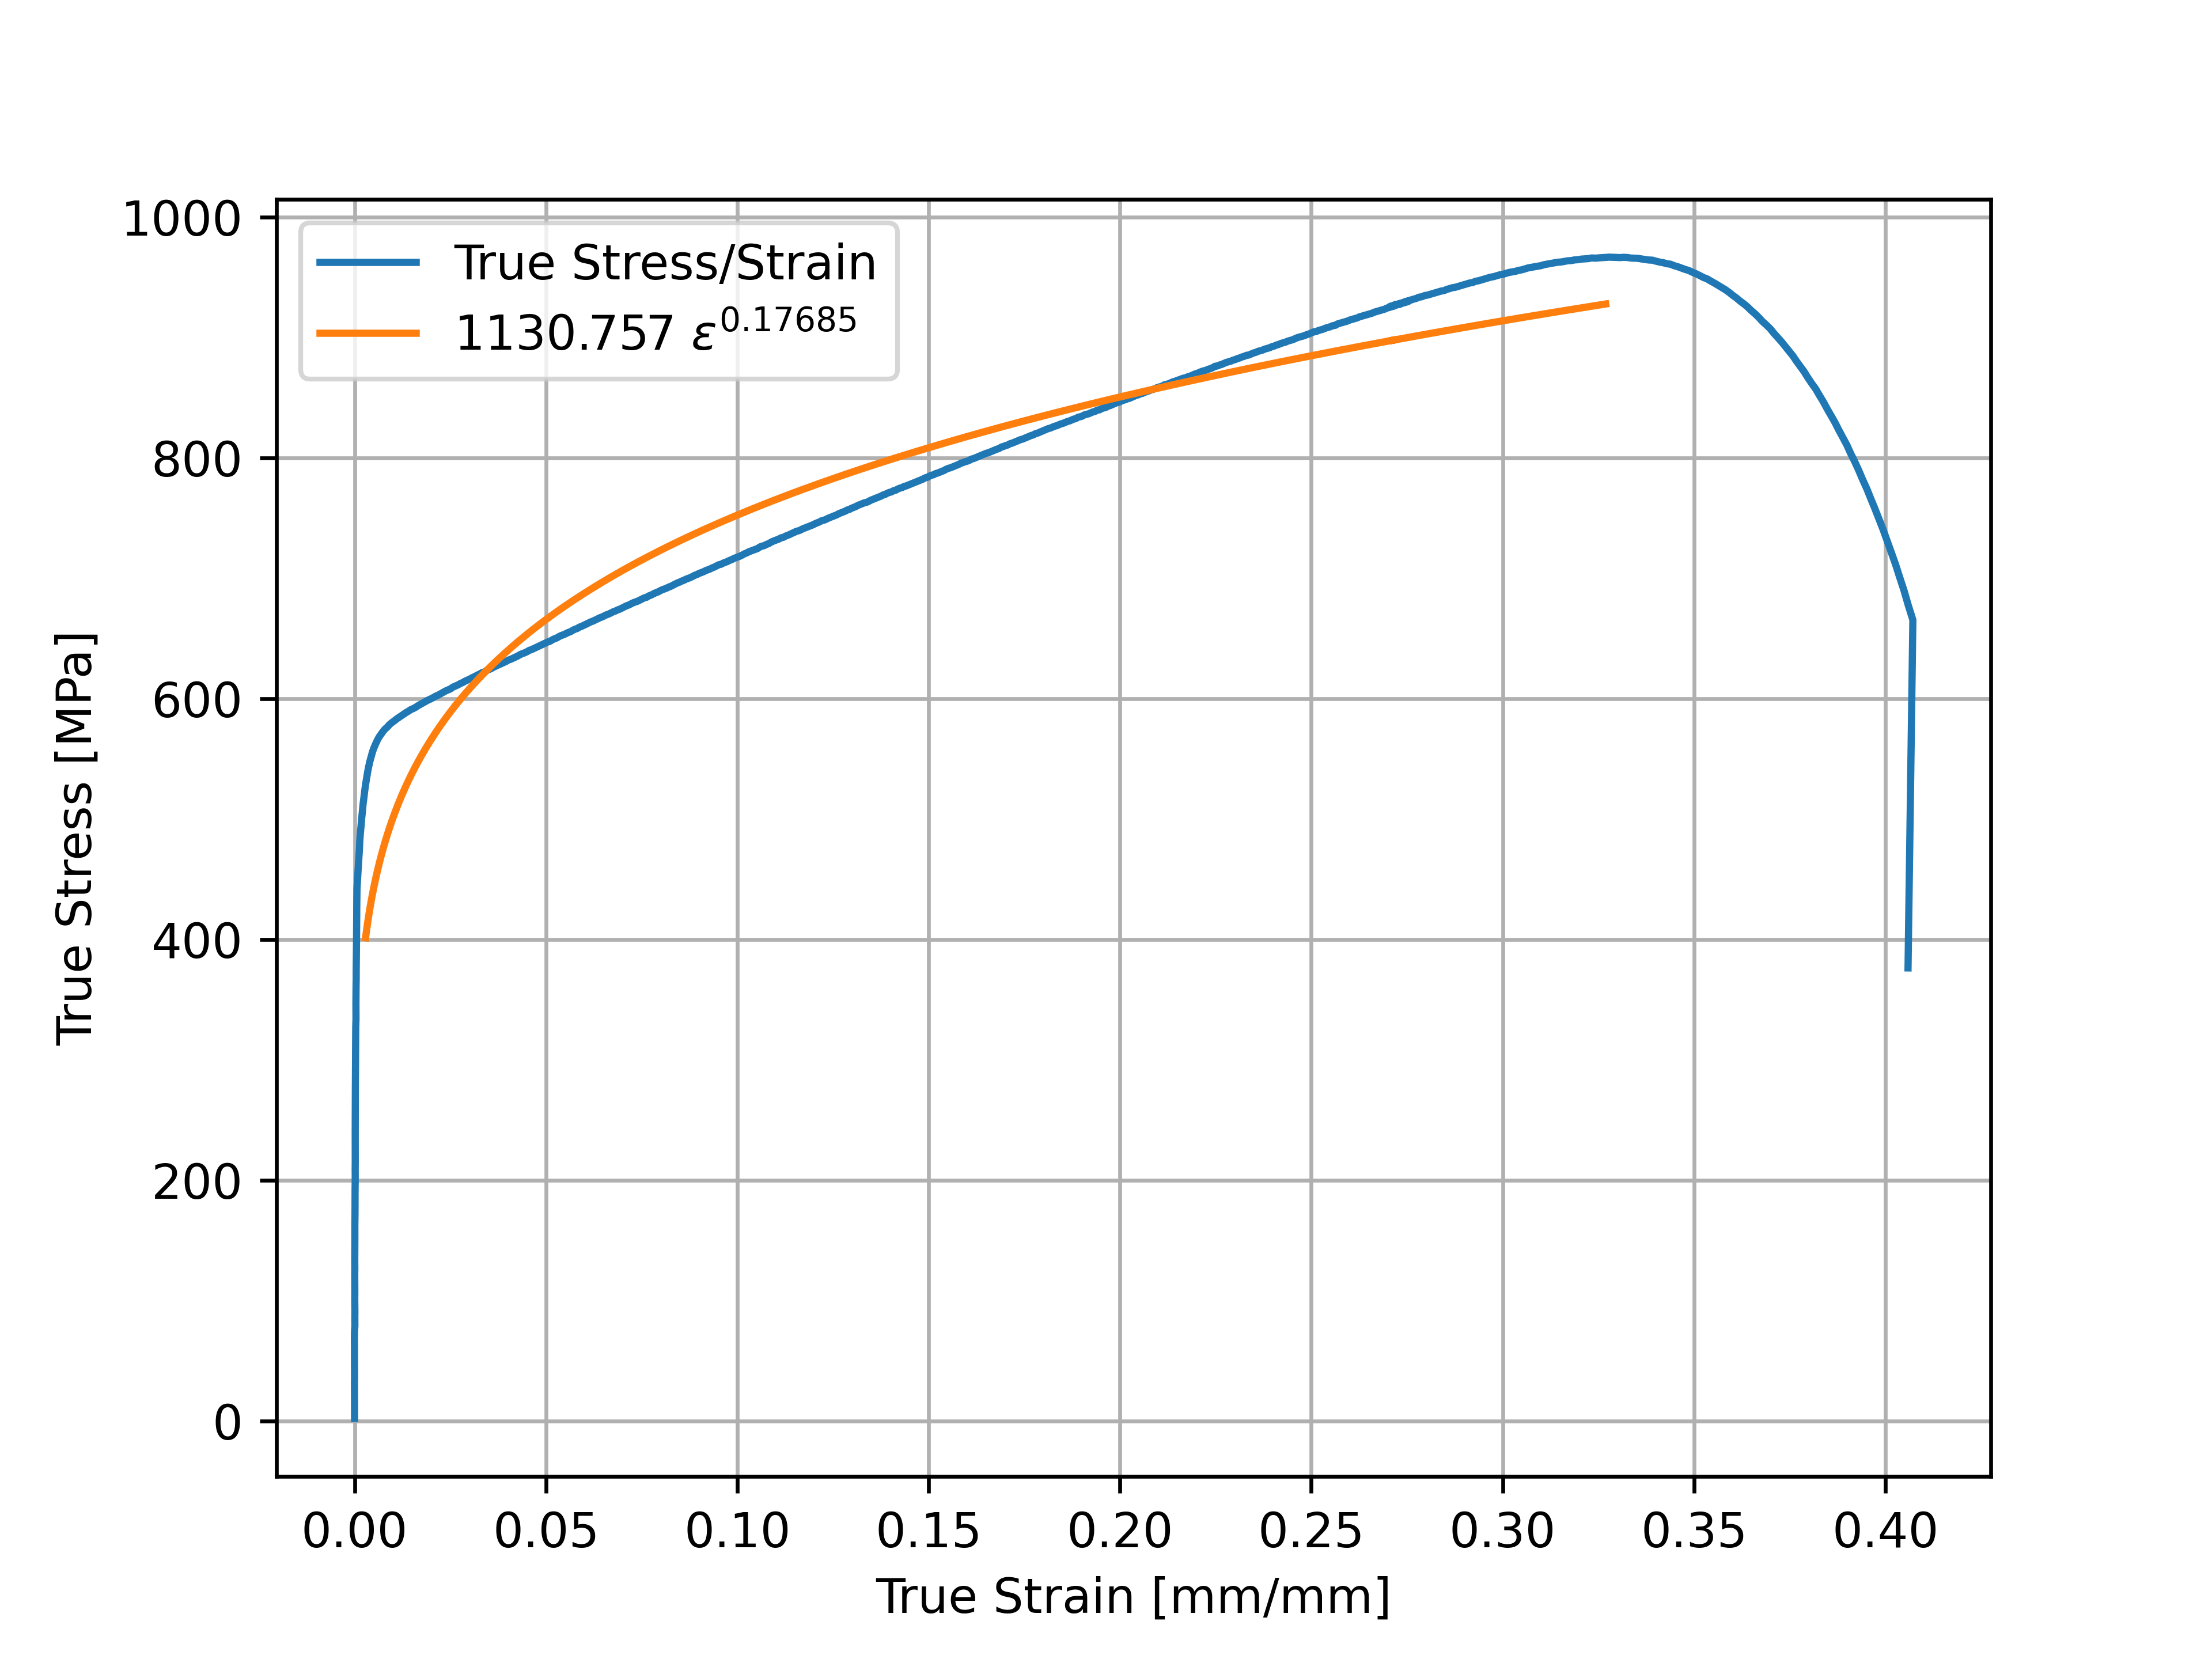
\includegraphics[width=0.5\linewidth]{plots/q5_fit.png}
    \caption{Power-Law fit of plastic deformation of 304 Stainless Steel}
    \label{fig:q5fit}
\end{figure}

\subsection{Question 6}


\section{Analysis and Discussion}

\newpage
\section{Conclusions}

\newpage
\section{References}
\printbibliography[heading=none]

\end{document}